\documentclass[10pt]{beamer}
\usetheme[progressbar=frametitle]{metropolis}
%use Fira
\usepackage{fontspec}
\setsansfont{Fira Sans}
\setmonofont{Fira Mono}
%fix textspacings...
\linespread{1.0} % Standard is 1.0, but Beamer often scales this
\setbeamerfont{block body}{size=\small} % Sometimes smaller font helps the 'density'
\addtobeamertemplate{block begin}{\setlength{\parskip}{0pt}}{}
\addtobeamertemplate{block begin}{}{\vspace{-0.5ex}} % add space after title
\addtobeamertemplate{block alerted begin}{}{\vspace{-0.5ex}} % Reduce space after title
\addtobeamertemplate{block example begin}{}{\vspace{-0.5ex}} % Reduce space after title
\setbeamercolor{block title alerted}{bg=} %remove background of alert blocks
%\addtobeamertemplate{block end}{\vspace{-1ex}}{}  % Reduce space after content

% Custom colors
\definecolor{customblue}{RGB}{79, 70, 229}
\definecolor{customlightblue}{RGB}{224, 231, 255}
\definecolor{customgreen}{RGB}{34, 197, 94}
\definecolor{customorange}{RGB}{249, 115, 22}
\definecolor{customred}{RGB}{239, 68, 68}

\definecolor{myDarkTeal}{RGB}{35, 55, 59}
\definecolor{myOrange}{RGB}{235, 129, 27}
\definecolor{myLightGreen}{RGB}{20,176,61}
\definecolor{myLightGray}{RGB}{250,250,250}

%\setbeamercolor{progress bar}{fg=customblue,bg=customlightblue}
%\setbeamercolor{frametitle}{bg=customblue}
%\setbeamercolor{alerted text}{fg=customblue}

\usepackage{tikz}
\usetikzlibrary{arrows.meta,positioning,shapes}


\usepackage{pgfplots}
\pgfplotsset{compat=newest}
%\pgfplotsset{compat=1.18}
\usetikzlibrary{fpu}

\usepackage[table]{xcolor}

\title{Day 3: Statistical Inference}
\subtitle{From Samples to Populations}
\author{}
\date{}

\begin{document}

% Title
\begin{frame}
\titlepage
\begin{center}
\textit{Using probability and likelihood to draw conclusions from data}
\end{center}
\end{frame}

% Overview
\begin{frame}{Today's Journey}

\begin{block}{Part I: Likelihood and Parameter Estimation}
\begin{itemize}
\item What is likelihood?
\item Maximum likelihood estimation
\item How certainty increases with sample size
\end{itemize}
\end{block}

\begin{block}{Part II: Confidence Intervals}
\begin{itemize}
\item Quantifying uncertainty in estimates
\item Construction and interpretation
\item Common misconceptions
\end{itemize}
\end{block}

\begin{block}{Part III: Hypothesis Testing}
\begin{itemize}
\item The logic of hypothesis testing
\item P-values and their interpretation
\item Type I/II errors and statistical power
\end{itemize}
\end{block}

\begin{block}{Part IV: Practical Issues}
\begin{itemize}
\item Effect sizes vs. statistical significance
\item Multiple testing problem
\item Reporting and interpretation
\end{itemize}
\end{block}
\end{frame}

% ============================================================================
% PART I: LIKELIHOOD
% ============================================================================

\begin{frame}
\begin{center}
\Huge \textbf{Part I} \\
\vspace{0.5cm}
\LARGE Likelihood and Parameter Estimation
\vspace{0.5cm}

\large \textit{How do we estimate parameters from data?}
\end{center}
\end{frame}

% The Estimation Problem
\begin{frame}{The Estimation Problem}

\textbf{Situation in biology:}
\begin{itemize}
\item Measure a sample of organisms/cells/genes
\item Want to estimate population parameter (mean, proportion, rate, etc.)
\item Have uncertainty due to sampling variability
\end{itemize}

\vspace{0.3cm}

\begin{exampleblock}{Examples}
\begin{itemize}
\item Disease prevalence: test 100 people, 15 positive → estimate p?
\item Mutation rate: sequence 1000 bp, find 3 mutations → estimate λ?
\item Mean enzyme activity: measure 20 samples → estimate μ?
\end{itemize}
\end{exampleblock}

\vspace{0.3cm}

\begin{alertblock}{Key Question}
Given data, which parameter value is \alert{most plausible}?
\end{alertblock}
\end{frame}

% Likelihood vs Probability
\begin{frame}{Likelihood vs. Probability}

\begin{columns}[T]
\begin{column}{0.48\textwidth}
\begin{block}{Probability}
\textbf{Given parameter, predict data}

\vspace{0.2cm}
$P(\text{data} \mid \theta)$

\vspace{0.2cm}
\textit{``If coin has p=0.5, \\
what's probability of 7 heads in 10 flips?''}

\vspace{0.2cm}
Forward reasoning: \\
parameter → data
\end{block}
\end{column}

\begin{column}{0.48\textwidth}
\begin{block}{Likelihood}
\textbf{Given data, evaluate parameter}

\vspace{0.2cm}
$L(\theta \mid \text{data})$

\vspace{0.2cm}
\textit{``Observed 7 heads in 10 flips, \\
how plausible is p=0.5?''}

\vspace{0.2cm}
Inverse reasoning: \\
data → parameter
\end{block}
\end{column}
\end{columns}

\vspace{0.5cm}

\begin{alertblock}{Key Insight}
\textbf{Same formula, different perspective!} \\
Likelihood treats data as fixed, parameter as variable
\end{alertblock}
\end{frame}

% Binomial Likelihood
\begin{frame}{Example: Binomial Likelihood}

\textbf{Setup:} Flip coin $n$ times, observe $x$ heads

\vspace{0.3cm}

\textbf{Likelihood function:}
$$L(p) = \binom{n}{x} p^x (1-p)^{n-x}$$

\vspace{0.3cm}

\begin{exampleblock}{Concrete Example: n=10, x=7}
$$L(p) = \binom{10}{7} p^7 (1-p)^3 = 120 \cdot p^7 (1-p)^3$$

\vspace{0.2cm}
Evaluate at different values:
\begin{itemize}
\item $L(0.5) = 120 \times 0.5^7 \times 0.5^3 = 0.117$
\item $L(0.7) = 120 \times 0.7^7 \times 0.3^3 = 0.267$ \alert{← highest!}
\item $L(0.9) = 120 \times 0.9^7 \times 0.1^3 = 0.057$
\end{itemize}
\end{exampleblock}

\vspace{0.2cm}
\textbf{Interpretation:} $p=0.7$ is most consistent with observing 7 heads in 10 flips
\end{frame}

% Likelihood Surface
\begin{frame}{Visualizing the Likelihood Surface}

\begin{center}
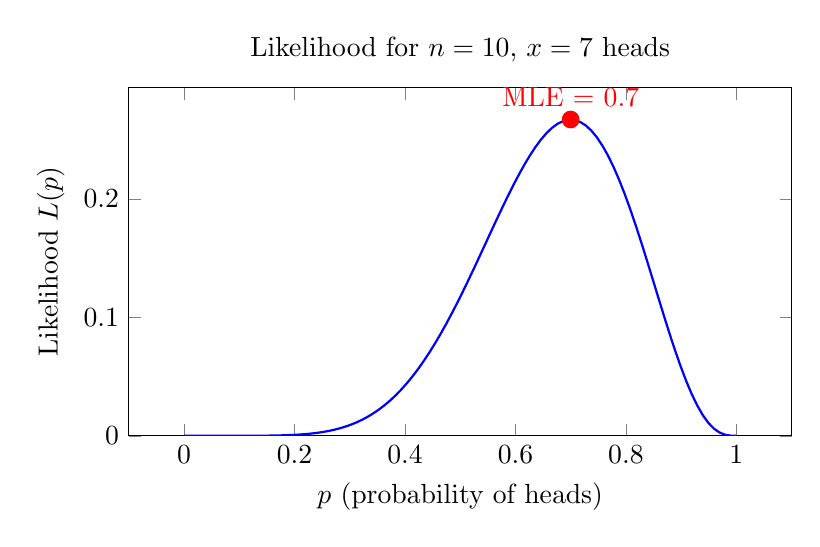
\begin{tikzpicture}
\begin{axis}[
    width=10cm,
    height=6cm,
    xlabel={$p$ (probability of heads)},
    ylabel={Likelihood $L(p)$},
    domain=0:1,
    samples=100,
    ymin=0,
    title={Likelihood for $n=10$, $x=7$ heads}
]
% Binomial likelihood: C(10,7) * p^7 * (1-p)^3
\addplot[thick, blue] {120 * x^7 * (1-x)^3};
\addplot[only marks, mark=*, mark size=3pt, red] coordinates {(0.7, 0.267)};
\node[above, red] at (axis cs:0.7,0.27) {MLE = 0.7};
\end{axis}
\end{tikzpicture}
\end{center}

\textbf{Observations:}
\begin{itemize}
\item Peak at $p = 7/10 = 0.7$ (intuitive!)
\item Fairly flat → lots of values plausible
\item Uncertainty due to small sample size
\end{itemize}
\end{frame}

% Maximum Likelihood Estimate
\begin{frame}{Maximum Likelihood Estimate (MLE)}

\begin{block}{Definition}
The \textbf{Maximum Likelihood Estimate (MLE)} is the parameter value that maximizes the likelihood function:
$$\hat{\theta}_{\text{MLE}} = \arg\max_{\theta} L(\theta \mid \text{data})$$
\end{block}

\vspace{0.3cm}

\textbf{For binomial:}
$$\hat{p} = \frac{x}{n}$$

(Can be shown by calculus: $\frac{dL}{dp} = 0$)

\vspace{0.3cm}

\textbf{Properties of MLE:}
\begin{itemize}
\item Intuitively sensible
\item Consistent: $\hat{\theta} \to \theta$ as $n \to \infty$
\item Asymptotically normal: $\hat{\theta} \sim N(\theta, \text{SE}^2)$ for large $n$
\item Basis for many statistical tests
\end{itemize}
\end{frame}

% Effect of Sample Size
\begin{frame}{Effect of Sample Size on Likelihood}

\textbf{Same proportion (70\% heads), different sample sizes:}

\vspace{0.3cm}

\begin{center}
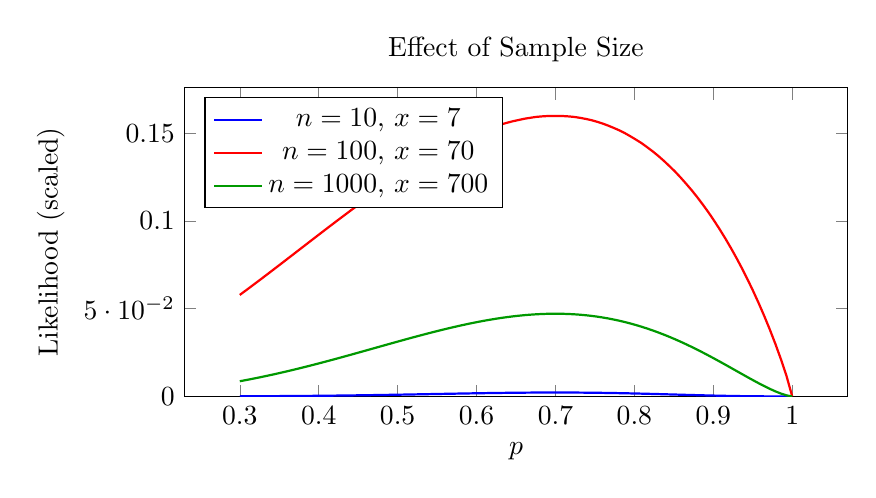
\begin{tikzpicture}
\begin{axis}[
    width=10cm,
    height=5.5cm,
    xlabel={$p$},
    ylabel={Likelihood (scaled)},
    domain=0.3:1,
    samples=100,
    legend pos=north west,
    ymin=0,
    title={Effect of Sample Size}
]
% n=10, x=7
\addplot[thick, blue] {x^7 * (1-x)^3};
\addlegendentry{$n=10$, $x=7$}

% n=100, x=70 (scaled to be visible)
\addplot[thick, red] {(x^70 * (1-x)^30)^0.03};
\addlegendentry{$n=100$, $x=70$}

% n=1000, x=700 (scaled to be visible)
\addplot[thick, green!60!black] {(x^700 * (1-x)^300)^0.005};
\addlegendentry{$n=1000$, $x=700$}
\end{axis}
\end{tikzpicture}
\end{center}

\textbf{Key observation:} Larger $n$ → sharper peak → more precision
\end{frame}

% Log-Likelihood
\begin{frame}{Log-Likelihood}

\textbf{Why use logarithms?}

\vspace{0.3cm}

\begin{block}{Definition}
$$\ell(\theta) = \log L(\theta)$$
\end{block}

\textbf{Advantages:}
\begin{enumerate}
\item Converts products to sums: $\log(ab) = \log a + \log b$
\item Easier to differentiate
\item Avoids numerical underflow (very small probabilities)
\item Same MLE: $\arg\max L = \arg\max \log L$
\end{enumerate}

\vspace{0.3cm}

\begin{exampleblock}{Binomial Log-Likelihood}
$$\ell(p) = \log\binom{n}{x} + x\log p + (n-x)\log(1-p)$$

Maximizing: $\frac{d\ell}{dp} = \frac{x}{p} - \frac{n-x}{1-p} = 0$ \\
Solving: $\hat{p} = \frac{x}{n}$
\end{exampleblock}
\end{frame}

% Biology Applications
\begin{frame}{Likelihood in Biology Research}

\textbf{Widespread applications:}

\vspace{0.3cm}

\begin{enumerate}
\item \textbf{Population genetics:} Estimate allele frequencies from genotype data

\vspace{0.2cm}
\item \textbf{Phylogenetics:} Find most likely evolutionary tree given DNA sequences

\vspace{0.2cm}
\item \textbf{Mark-recapture:} Estimate population size from capture data

\vspace{0.2cm}
\item \textbf{GLMs:} Generalized linear models (Poisson regression, logistic regression)

\vspace{0.2cm}
\item \textbf{Mixed models:} Estimate variance components in nested/hierarchical data

\vspace{0.2cm}
\item \textbf{Survival analysis:} Estimate hazard rates from time-to-event data
\end{enumerate}

\vspace{0.3cm}

\begin{alertblock}{}
\centering
MLE is the foundation of modern statistical inference!
\end{alertblock}
\end{frame}

% ============================================================================
% PART II: CONFIDENCE INTERVALS
% ============================================================================

\begin{frame}
\begin{center}
\Huge \textbf{Part II} \\
\vspace{0.5cm}
\LARGE Confidence Intervals
\vspace{0.5cm}

\large \textit{Quantifying uncertainty in our estimates}
\end{center}
\end{frame}

% The Logic
\begin{frame}{The Logic of Confidence Intervals}

\textbf{Recall from Day 2 (CLT):}
\begin{itemize}
\item Sample mean $\bar{x}$ varies across samples
\item Sampling distribution: $\bar{X} \sim N(\mu, \sigma^2/n)$
\item Standard Error: $SE = \sigma/\sqrt{n}$
\item 95\% of sample means fall within $\mu \pm 1.96 \times SE$
\end{itemize}

\vspace{0.3cm}

\begin{alertblock}{The Flip}
\textbf{Yesterday:} Given $\mu$, where is $\bar{x}$?

\textbf{Today:} Given $\bar{x}$, where is $\mu$?
\end{alertblock}

\vspace{0.3cm}

\textbf{Confidence Interval:}
$$\bar{x} \pm 1.96 \times SE$$

This interval will contain $\mu$ for 95\% of samples
\end{frame}

% Construction
\begin{frame}{Constructing a 95\% Confidence Interval}

\textbf{Case 1: Known $\sigma$ (rare in practice)}

$$\text{CI} = \bar{x} \pm 1.96 \times \frac{\sigma}{\sqrt{n}}$$

\vspace{0.3cm}

\textbf{Case 2: Unknown $\sigma$ (usual case)}

Use sample SD $s$ and $t$-distribution:
$$\text{CI} = \bar{x} \pm t_{\alpha/2, n-1} \times \frac{s}{\sqrt{n}}$$

where $t_{\alpha/2, n-1}$ is the critical value from $t$-distribution with $n-1$ degrees of freedom

\vspace{0.3cm}

\begin{exampleblock}{Example: Blood Pressure}
$n=25$, $\bar{x}=122$ mmHg, $s=15$ mmHg

\vspace{0.2cm}
$SE = 15/\sqrt{25} = 3$ mmHg \\
$t_{0.025, 24} = 2.064$ \\
$\text{CI} = 122 \pm 2.064 \times 3 = 122 \pm 6.2 = [115.8, 128.2]$
\end{exampleblock}
\end{frame}

% Interpretation
\begin{frame}{Interpreting Confidence Intervals}

\begin{block}{CORRECT Interpretation}
``We are 95\% confident that the interval $[115.8, 128.2]$ contains the true population mean $\mu$.''

\vspace{0.2cm}
Or: ``If we repeated this procedure many times, 95\% of the intervals would contain $\mu$.''
\end{block}

\vspace{0.3cm}

\begin{alertblock}{INCORRECT Interpretations}
\begin{itemize}
\item ✗ ``There's a 95\% probability that $\mu$ is in this interval'' \\
\small (Frequentist: $\mu$ is fixed, not random)

\item ✗ ``95\% of the data falls in this interval'' \\
\small (No! CI is about the parameter, not individual observations)

\item ✗ ``This specific interval has 95\% chance of containing $\mu$'' \\
\small (Once computed, either it does or doesn't—probability is about the procedure)
\end{itemize}
\end{alertblock}
\end{frame}

% Visualization
\begin{frame}{Visualizing Confidence Intervals}

\textbf{Simulation: 20 different samples, each gets a CI}

\vspace{0.2cm}

\begin{center}
\begin{tikzpicture}[scale=0.8]
\draw[thick, dashed, red] (5, 0) -- (5, 11) node[above] {True $\mu$};

\foreach \y/\color in {1/blue, 2/blue, 3/blue, 4/blue, 5/blue, 6/blue, 7/blue, 8/blue, 9/blue, 10/blue, 11/blue, 12/blue, 13/blue, 14/blue, 15/red, 16/blue, 17/blue, 18/blue, 19/blue, 20/blue} {
  \pgfmathsetmacro{\xmean}{5 + 0.6*rand}
  \pgfmathsetmacro{\xlower}{\xmean - 1}
  \pgfmathsetmacro{\xupper}{\xmean + 1}
  
  \draw[\color, thick] (\xlower, \y*0.5) -- (\xupper, \y*0.5);
  \fill[\color] (\xmean, \y*0.5) circle (2pt);
}

\draw[<->] (2, -0.5) -- (8, -0.5);
\node at (5, -1) {Parameter value};
\node[left] at (0, 5.5) {Different samples};
\end{tikzpicture}
\end{center}

\small \textcolor{blue}{19 intervals (95\%) contain $\mu$} \\
\textcolor{red}{1 interval (5\%) misses $\mu$}
\end{frame}

% Factors Affecting Width
\begin{frame}{Factors Affecting CI Width}

$$\text{Width} = 2 \times t_{\alpha/2} \times \frac{s}{\sqrt{n}}$$

\vspace{0.3cm}

\textbf{Narrower intervals (more precision) when:}

\begin{enumerate}
\item \textbf{Larger sample size ($n$):} Width $\propto 1/\sqrt{n}$
\begin{itemize}
\item Double the sample → width decreases by $\sqrt{2}$
\item To halve width, need 4× the data!
\end{itemize}

\vspace{0.2cm}
\item \textbf{Smaller variability ($s$):} More consistent measurements

\vspace{0.2cm}
\item \textbf{Lower confidence level:} 90\% CI narrower than 95\% CI
\begin{itemize}
\item But: trade-off between precision and confidence
\end{itemize}
\end{enumerate}

\vspace{0.3cm}

\begin{alertblock}{}
\centering
Can't have high precision and high confidence with small samples!
\end{alertblock}
\end{frame}

% Likelihood-based CI
\begin{frame}{Likelihood-Based Confidence Intervals}

\textbf{Alternative approach using likelihood:}

\vspace{0.3cm}

\begin{block}{Profile Likelihood CI}
Include all parameter values $\theta$ where:
$$-2[\ell(\theta) - \ell(\hat{\theta})] < \chi^2_{\alpha, 1}$$

For 95\% CI: $\chi^2_{0.05, 1} = 3.84$

\vspace{0.2cm}
Or approximately: $\ell(\theta) > \ell(\hat{\theta}) - 1.92$
\end{block}

\vspace{0.3cm}

\textbf{Advantages:}
\begin{itemize}
\item More accurate for small samples or non-normal distributions
\item Automatically respects parameter bounds (e.g., $p \in [0,1]$)
\item Basis for likelihood ratio tests
\end{itemize}

\vspace{0.2cm}

\textbf{In practice:} For large $n$, Wald and profile CIs are similar
\end{frame}

% ============================================================================
% PART III: HYPOTHESIS TESTING
% ============================================================================

\begin{frame}
\begin{center}
\Huge \textbf{Part III} \\
\vspace{0.5cm}
\LARGE Hypothesis Testing
\vspace{0.5cm}

\large \textit{Is the effect real, or just chance?}
\end{center}
\end{frame}

% The Logic
\begin{frame}{The Logic of Hypothesis Testing}

\textbf{Scientific question:} Does drug reduce blood pressure?

\vspace{0.3cm}

\textbf{Statistical approach:} Proof by contradiction

\begin{enumerate}
\item \textbf{Assume} drug has no effect (null hypothesis $H_0$)
\item Calculate: How likely is our observed data under $H_0$?
\item If very unlikely, reject $H_0$ (evidence for effect)
\item If not unlikely, fail to reject $H_0$ (insufficient evidence)
\end{enumerate}

\vspace{0.3cm}

\begin{alertblock}{Key Insight}
We \alert{never prove $H_0$ is true}—we only assess if data are \alert{incompatible} with $H_0$
\end{alertblock}

\vspace{0.2cm}

\textit{``Absence of evidence is not evidence of absence''}
\end{frame}

% Hypotheses
\begin{frame}{Null and Alternative Hypotheses}

\begin{block}{Null Hypothesis ($H_0$)}
Statement of \textbf{no effect} or \textbf{no difference}
\begin{itemize}
\item $H_0: \mu = \mu_0$ (mean equals specific value)
\item $H_0: \mu_1 = \mu_2$ (two groups have same mean)
\item $H_0: p = 0.5$ (proportion equals 0.5)
\end{itemize}
\end{block}

\begin{block}{Alternative Hypothesis ($H_A$ or $H_1$)}
What we suspect is true; contradicts $H_0$
\begin{itemize}
\item $H_A: \mu \neq \mu_0$ (two-sided: different in either direction)
\item $H_A: \mu > \mu_0$ (one-sided: specifically greater)
\item $H_A: \mu < \mu_0$ (one-sided: specifically less)
\end{itemize}
\end{block}

\vspace{0.2cm}

\begin{exampleblock}{Biology Example}
Test if knockout mice weigh less than wild-type: \\
$H_0: \mu_{\text{knockout}} = \mu_{\text{WT}}$ \quad vs. \quad $H_A: \mu_{\text{knockout}} < \mu_{\text{WT}}$
\end{exampleblock}
\end{frame}

% Test Statistic
\begin{frame}{Test Statistics}

\textbf{Need a number that measures deviation from $H_0$}

\vspace{0.3cm}

\begin{block}{General Form}
$$\text{Test Statistic} = \frac{\text{Estimate} - \text{Hypothesized value}}{\text{Standard Error}}$$
\end{block}

\vspace{0.3cm}

\textbf{Common test statistics:}

\begin{itemize}
\item \textbf{Z-statistic:} $Z = \frac{\bar{x} - \mu_0}{\sigma/\sqrt{n}}$ \quad (known $\sigma$)

\vspace{0.2cm}
\item \textbf{t-statistic:} $t = \frac{\bar{x} - \mu_0}{s/\sqrt{n}}$ \quad (unknown $\sigma$, use $s$)

\vspace{0.2cm}
\item \textbf{Two-sample t:} $t = \frac{\bar{x}_1 - \bar{x}_2}{\text{SE}_{\text{diff}}}$
\end{itemize}

\vspace{0.3cm}

\textbf{Under $H_0$:} Test statistic follows known distribution \\
\small (Z-distribution, t-distribution, etc.)
\end{frame}

% P-values
\begin{frame}{P-values}

\begin{block}{Definition}
\textbf{P-value} = Probability of observing data as extreme as (or more extreme than) what we actually observed, \alert{if $H_0$ were true}
$$p\text{-value} = P(\text{data as extreme} \mid H_0 \text{ true})$$
\end{block}

\vspace{0.3cm}

\textbf{Interpretation:}
\begin{itemize}
\item \textbf{Small p-value} (e.g., $p < 0.05$): Data are \alert{incompatible} with $H_0$ → reject $H_0$
\item \textbf{Large p-value} (e.g., $p > 0.05$): Data are \alert{consistent} with $H_0$ → fail to reject $H_0$
\end{itemize}

\vspace{0.3cm}

\begin{exampleblock}{Example}
$t = 2.5$, $p = 0.02$

\vspace{0.2cm}
\textit{``If there were truly no effect, we'd see a test statistic this large (or larger) only 2\% of the time. Since this is unlikely, we reject $H_0$."}
\end{exampleblock}
\end{frame}

% P-value Visualization
\begin{frame}{Visualizing P-values}

\textbf{Two-sided test:} $H_0: \mu = 0$, observed $t = 2.5$

\vspace{0.2cm}

\begin{center}
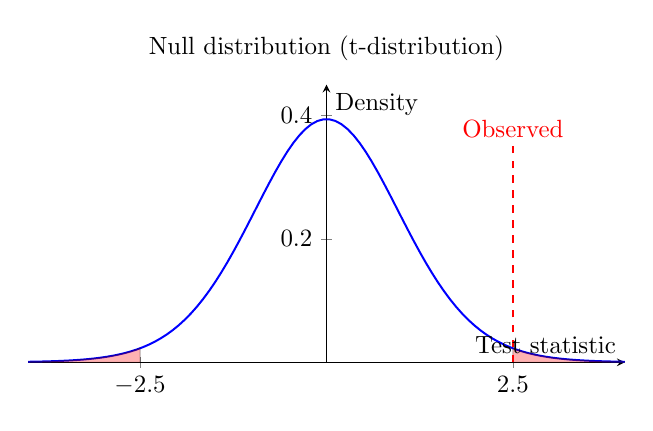
\begin{tikzpicture}[scale=0.9]
\begin{axis}[
    width=10cm,
    height=5.5cm,
    domain=-4:4,
    samples=100,
    xlabel={Test statistic},
    ylabel={Density},
    axis lines=center,
    ymin=0, ymax=0.45,
    xtick={-2.5, 0, 2.5},
    xticklabels={$-2.5$, $0$, $2.5$},
    title={Null distribution (t-distribution)}
]
% t-distribution with df=20
\addplot[thick, blue, domain=-4:4] {1133278.38/(sqrt(20*pi)*362880) * (1 + x^2/20)^(-10.5)};

% Shade tails
\addplot[fill=red, opacity=0.3, domain=2.5:4] {1133278.38/(sqrt(20*pi)*362880) * (1 + x^2/20)^(-10.5)} \closedcycle;
\addplot[fill=red, opacity=0.3, domain=-4:-2.5] {1133278.38/(sqrt(20*pi)*362880) * (1 + x^2/20)^(-10.5)} \closedcycle;

% Mark observed value
\draw[thick, red, dashed] (axis cs:2.5,0) -- (axis cs:2.5,0.35);
\node[above, red] at (axis cs:2.5,0.35) {Observed};
\end{axis}
\end{tikzpicture}
\end{center}

\small \textcolor{red}{Shaded area = p-value} (probability in both tails)
\end{frame}

% What P-values Are NOT
\begin{frame}{What P-values Are NOT}

\begin{alertblock}{Common Misconceptions}

\textbf{P-value is NOT:}

\begin{itemize}
\item ✗ Probability that $H_0$ is true \\
\small (We condition on $H_0$ being true to calculate p!)

\vspace{0.2cm}
\item ✗ Probability that results are due to chance \\
\small (Everything has chance involved; p quantifies compatibility with $H_0$)

\vspace{0.2cm}
\item ✗ Probability of making a mistake \\
\small (That's $\alpha$, not p)

\vspace{0.2cm}
\item ✗ Size of the effect \\
\small (Large effect with large n → small p; small effect with huge n → small p)

\vspace{0.2cm}
\item ✗ Importance of the finding \\
\small (Statistical significance $\neq$ practical significance)
\end{itemize}
\end{alertblock}

\vspace{0.2cm}

\textbf{P-value IS:} Measure of compatibility between data and $H_0$
\end{frame}

% Decision Rule
\begin{frame}{Decision Rules and Significance Level}

\begin{block}{Significance Level ($\alpha$)}
Threshold for rejecting $H_0$ (conventionally 0.05)

\vspace{0.2cm}
\textbf{Decision rule:}
\begin{itemize}
\item If $p < \alpha$: Reject $H_0$ (result is ``statistically significant'')
\item If $p \geq \alpha$: Fail to reject $H_0$ (result is ``not significant'')
\end{itemize}
\end{block}

\vspace{0.3cm}

\begin{alertblock}{Important Notes}
\begin{itemize}
\item $\alpha = 0.05$ is arbitrary! (R.A. Fisher's convention)
\item Don't treat $p = 0.049$ differently from $p = 0.051$
\item Better: Report exact p-value, let readers judge
\item Even better: Report effect sizes with CIs!
\end{itemize}
\end{alertblock}

\vspace{0.2cm}

\textbf{Modern practice:} De-emphasize ``significant'' / ``not significant'' binary
\end{frame}

%%%%%%%%%%%%%%%%%%%%%%%%%%%%%%%%%%%%%%%%%
\begin{frame}{One sided vs Two-sided tests}
\begin{columns}[T]
	\begin{column}{.48\textwidth}

\begin{block}{Two-Sided}
$H_0: \mu = \mu_0$ \\
$H_A: \mu \neq \mu_0$ (or $\leq$)

\vspace{0.2cm}
Detect difference in \textbf{any direction}

\vspace{0.2cm}
P-value: area in both tails

\vspace{0.2cm}
\textbf{Use when:} No a priori reason to expect a specific direction
\end{block}
\end{column}

\begin{column}{0.48\textwidth}
\begin{block}{One-Sided}
$H_0: \mu = \mu_0$ \\
$H_A: \mu > \mu_0$ (or $\leq$)

\vspace{0.2cm}
Detect difference in \textbf{one direction}

\vspace{0.2cm}
P-value: area in one tail

\vspace{0.2cm}
\textbf{Use when:} Strong a priori reason to expect specific direction
\end{block}
\end{column}
\end{columns}

\vspace{0.2cm}

\begin{block}{Example}
	\small	
Test if drug \emph{reduces} blood pressure (not just changes it): \\
$H_0: \mu_{\text{drug}} = \mu_{\text{placebo}}$ vs. $H_A: \mu_{\text{drug}} < \mu_{\text{placebo}}$

%\vspace{0.2cm}
One-sided p-value = half of two-sided p-value (if effect in predicted direction)
\end{block}

\vspace{0.2cm}

\begin{alertblock}{Caution}
Don't choose one-sided after seeing data! Inflates Type I error rate
\end{alertblock}
\end{frame}

% Type I and II Errors
\begin{frame}{Type I and Type II Errors}

\begin{center}
\begin{tabular}{|l|c|c|}
\hline
\textbf{} & \textbf{$H_0$ True} & \textbf{$H_0$ False} \\
\hline
\textbf{Reject $H_0$} & \cellcolor{red!30} Type I Error & \cellcolor{green!30} Correct \\
& \cellcolor{red!30} (False Positive) & \cellcolor{green!30} (True Positive) \\
& \cellcolor{red!30} Probability = $\alpha$ & \cellcolor{green!30} Probability = Power \\
\hline
\textbf{Fail to Reject $H_0$} & \cellcolor{green!30} Correct & \cellcolor{orange!30} Type II Error \\
& \cellcolor{green!30} (True Negative) & \cellcolor{orange!30} (False Negative) \\
& \cellcolor{green!30} Probability = $1-\alpha$ & \cellcolor{orange!30} Probability = $\beta$ \\
\hline
\end{tabular}
\end{center}

\vspace{0.4cm}

\begin{block}{Definitions}
\begin{itemize}
\item \textbf{Type I Error ($\alpha$):} Reject $H_0$ when it's true (false alarm)
\item \textbf{Type II Error ($\beta$):} Fail to reject $H_0$ when it's false (miss)
\item \textbf{Power ($1-\beta$):} Correctly reject $H_0$ when it's false (detect real effect)
\end{itemize}
\end{block}
\end{frame}

% Trade-offs
\begin{frame}{Trade-offs Between Error Types}

\textbf{The dilemma:} Can't minimize both errors simultaneously!

\vspace{0.3cm}

\begin{itemize}
\item \textbf{Decrease $\alpha$} (be more conservative): \\
→ Fewer false positives, but more false negatives (lower power)

\vspace{0.2cm}
\item \textbf{Increase sample size $n$}: \\
→ Decreases both $\alpha$ and $\beta$ (increases power)

\vspace{0.2cm}
\item \textbf{Convention:} Fix $\alpha = 0.05$, then maximize power
\end{itemize}

\vspace{0.3cm}

\begin{exampleblock}{Medical Testing Analogy}
\begin{itemize}
\item Type I error: False positive (healthy person diagnosed as sick)
\item Type II error: False negative (sick person diagnosed as healthy)
\item Which is worse depends on context (cancer screening vs. common cold)
\end{itemize}
\end{exampleblock}

\vspace{0.2cm}

\textbf{In biology:} Type II errors often more common due to small samples
\end{frame}

% Statistical Power
\begin{frame}{Statistical Power}

\begin{block}{Definition}
\textbf{Power} = Probability of detecting an effect when it truly exists
$\text{Power} = 1 - \beta = P(\text{reject } H_0 \mid H_0 \text{ false})$
\end{block}

\vspace{0.3cm}

\textbf{Power depends on:}
\begin{enumerate}
\item \textbf{Effect size:} Larger effect → easier to detect → higher power
\item \textbf{Sample size ($n$):} Larger $n$ → higher power
\item \textbf{Significance level ($\alpha$):} Larger $\alpha$ → higher power (but more Type I errors)
\item \textbf{Variability ($\sigma$):} Lower $\sigma$ → higher power
\end{enumerate}

\vspace{0.3cm}

\begin{alertblock}{Rule of Thumb}
Aim for power $\geq 0.80$ (80\% chance of detecting real effect)

\vspace{0.2cm}
Many published studies are \alert{underpowered} (power $< 0.50$)!
\end{alertblock}
\end{frame}

% Power Analysis
\begin{frame}{Power Analysis: Planning Sample Size}

\textbf{Before collecting data, ask:} How many samples do I need?

\vspace{0.3cm}

\begin{block}{Power Analysis}
Calculate required $n$ given:
\begin{itemize}
\item Desired power (typically 0.80)
\item Significance level $\alpha$ (typically 0.05)
\item Expected effect size (from pilot data or literature)
\item Expected variability
\end{itemize}
\end{block}

\vspace{0.3cm}

\begin{exampleblock}{Example: Two-Sample t-test}
Compare treatment vs. control mean enzyme activity

\vspace{0.2cm}
\textbf{Given:} \\
- Expected difference: 5 units \\
- Expected SD: 8 units \\
- Desired power: 0.80, $\alpha = 0.05$

\vspace{0.2cm}
\textbf{Required:} $n \approx 52$ per group (total 104)
\end{exampleblock}

\vspace{0.2cm}

\textbf{Software:} G*Power, R packages (pwr), online calculators
\end{frame}

% ============================================================================
% PART IV: PRACTICAL ISSUES
% ============================================================================

\begin{frame}
\begin{center}
\Huge \textbf{Part IV} \\
\vspace{0.5cm}
\LARGE Practical Issues in Inference
\vspace{0.5cm}

\large \textit{Beyond p < 0.05}
\end{center}
\end{frame}

% Effect Sizes
\begin{frame}{Effect Sizes: Size Matters!}

\begin{alertblock}{Critical Distinction}
\textbf{Statistical significance} $\neq$ \textbf{Practical importance}
\end{alertblock}

\vspace{0.3cm}

\textbf{Why p-values aren't enough:}
\begin{itemize}
\item With large $n$, tiny effects become "significant"
\item With small $n$, large effects may not reach significance
\item P-values conflate effect size and sample size
\end{itemize}

\vspace{0.3cm}

\begin{block}{Effect Sizes}
Quantify the \textbf{magnitude} of the effect (independent of sample size)

\textbf{Common measures:}
\begin{itemize}
\item \textbf{Cohen's d:} $d = \frac{\bar{x}_1 - \bar{x}_2}{s_{\text{pooled}}}$ (standardized difference)
\item \textbf{Correlation:} $r$ (strength of relationship)
\item \textbf{Odds ratio, Risk ratio:} For binary outcomes
\end{itemize}
\end{block}
\end{frame}

% Example
\begin{frame}{Example: Statistical vs. Biological Significance}

\begin{exampleblock}{Scenario A: Large sample, tiny effect}
Compare gene expression in treatment vs. control

\vspace{0.2cm}
$n = 10,000$ per group, $\bar{x}_1 - \bar{x}_2 = 0.05$ (1\% change), $p < 0.0001$

\vspace{0.2cm}
\textbf{Conclusion:} Statistically significant, but biologically trivial!
\end{exampleblock}

\vspace{0.3cm}

\begin{exampleblock}{Scenario B: Small sample, large effect}
Compare tumor size in mice

\vspace{0.2cm}
$n = 5$ per group, tumor reduction = 40\%, $p = 0.12$

\vspace{0.2cm}
\textbf{Conclusion:} Not statistically significant, but effect size suggests important biology worth investigating further!
\end{exampleblock}

\vspace{0.3cm}

\begin{alertblock}{}
\centering
\textbf{Always report effect sizes with confidence intervals!}
\end{alertblock}
\end{frame}

% Multiple Testing
\begin{frame}{The Multiple Testing Problem}

\begin{alertblock}{The Problem}
Test many hypotheses → inflated false positive rate
\end{alertblock}

\vspace{0.3cm}

\textbf{Example:} Test 1000 genes for differential expression
\begin{itemize}
\item If \emph{none} are truly differentially expressed
\item Using $\alpha = 0.05$, expect $1000 \times 0.05 = 50$ false positives!
\end{itemize}

\vspace{0.3cm}

\textbf{Solutions:}

\begin{block}{Bonferroni Correction}
Divide $\alpha$ by number of tests: $\alpha_{\text{adj}} = \alpha / m$

Very conservative (low power for large $m$)
\end{block}

\begin{block}{False Discovery Rate (FDR)}
Control proportion of false positives among rejections

\vspace{0.2cm}
Benjamini-Hochberg procedure: More powerful than Bonferroni \\
\small (Standard in genomics: RNA-seq, GWAS, etc.)
\end{block}
\end{frame}

% Assumptions
\begin{frame}{Checking Assumptions}

\textbf{All tests make assumptions—violate them at your peril!}

\vspace{0.3cm}

\begin{block}{Common Assumptions for t-tests}
\begin{enumerate}
\item \textbf{Independence:} Observations independent of each other
\item \textbf{Normality:} Data (or residuals) approximately normal
\item \textbf{Equal variances:} (for two-sample t-test)
\end{enumerate}
\end{block}

\vspace{0.3cm}

\textbf{When assumptions violated:}
\begin{itemize}
\item \textbf{Independence:} Very serious! Use mixed models, GEE
\item \textbf{Normality:} Less critical for large $n$ (CLT!), but check with Q-Q plots
\item \textbf{Equal variances:} Use Welch's t-test (unequal variances version)
\end{itemize}

\vspace{0.3cm}

\textbf{Non-parametric alternatives:}
\begin{itemize}
\item Wilcoxon rank-sum test (instead of two-sample t-test)
\item Kruskal-Wallis test (instead of ANOVA)
\end{itemize}
\end{frame}

% What to Report
\begin{frame}{What to Report in Your Papers}

\begin{block}{Minimum Requirements}
\begin{enumerate}
\item \textbf{Sample sizes} for all groups
\item \textbf{Effect sizes} with 95\% confidence intervals
\item \textbf{Exact p-values} (not just $p < 0.05$), or at least $p < 0.001$
\item \textbf{Which test} was used and why
\item \textbf{Assumptions checked} and results
\item \textbf{Multiple testing corrections} applied (if any)
\end{enumerate}
\end{block}

\vspace{0.3cm}

\begin{exampleblock}{Good Example}
\textit{``Treatment group (n=25) had significantly lower blood pressure than control (n=23): mean difference = -12.3 mmHg (95\% CI: -18.5 to -6.1), t(46) = -4.02, p < 0.001, Cohen's d = 1.18.''}
\end{exampleblock}

\vspace{0.2cm}

\begin{alertblock}{Bad Example}
\textit{``Treatment significantly reduced blood pressure (p < 0.05).''}
\end{alertblock}
\end{frame}

% Common Mistakes
\begin{frame}{Common Mistakes and Misinterpretations}

\begin{enumerate}
\item \textbf{P-hacking:} Trying analyses until $p < 0.05$ \\
\small \textit{Solution:} Pre-register analysis plan

\vspace{0.2cm}
\item \textbf{Conflating significance with importance} \\
\small \textit{Solution:} Always report effect sizes

\vspace{0.2cm}
\item \textbf{Treating $p = 0.049$ differently from $p = 0.051$} \\
\small \textit{Solution:} Avoid dichotomous thinking

\vspace{0.2cm}
\item \textbf{Concluding "no difference" from $p > 0.05$} \\
\small \textit{Solution:} Check power; "absence of evidence $\neq$ evidence of absence"

\vspace{0.2cm}
\item \textbf{Multiple testing without correction} \\
\small \textit{Solution:} Use Bonferroni or FDR control

\vspace{0.2cm}
\item \textbf{Ignoring violated assumptions} \\
\small \textit{Solution:} Check assumptions, use robust methods

\vspace{0.2cm}
\item \textbf{Confusing practical and statistical significance} \\
\small \textit{Solution:} Consider biological context
\end{enumerate}
\end{frame}

% Modern Recommendations
\begin{frame}{Modern Statistical Practice}

\textbf{The field is moving beyond rigid $p < 0.05$ thinking:}

\vspace{0.3cm}

\begin{block}{ASA Statement on P-values (2016)}
\begin{itemize}
\item P-values can indicate incompatibility with a specified model
\item P-values do not measure probability that hypothesis is true
\item Scientific conclusions should not be based only on p-values
\item P-values don't measure size or importance of an effect
\item By itself, a p-value doesn't provide good evidence
\end{itemize}
\end{block}

\vspace{0.3cm}

\textbf{Better practices:}
\begin{itemize}
\item Report effect sizes with CIs
\item Use estimation rather than just testing
\item Pre-register analyses
\item Make data and code available
\item Replicate findings
\item Consider Bayesian approaches
\end{itemize}
\end{frame}

% Connection to Day 1
\begin{frame}{Connecting Back to Day 1: Philosophy}

\textbf{Remember the philosophical foundations?}

\vspace{0.3cm}

\begin{itemize}
\item \textbf{Induction problem:} We can never be certain—CIs and p-values quantify uncertainty

\vspace{0.2cm}
\item \textbf{Models vs. reality:} Hypothesis tests are models of decision-making

\vspace{0.2cm}
\item \textbf{Objectivity vs. subjectivity:} Multiple testing, researcher degrees of freedom

\vspace{0.2cm}
\item \textbf{Replication crisis:} P-hacking, publication bias, low power

\vspace{0.2cm}
\item \textbf{Effect sizes matter:} Prediction vs. explanation tension
\end{itemize}

\vspace{0.4cm}

\begin{alertblock}{}
\centering
\textbf{Statistics is not just formulas—} \\
it's a framework for reasoning under uncertainty
\end{alertblock}
\end{frame}

% Summary
\begin{frame}{Summary: Key Takeaways}

\begin{enumerate}
\item \textbf{Likelihood} provides a principled way to estimate parameters from data

\vspace{0.2cm}
\item \textbf{Confidence intervals} quantify uncertainty—not just point estimates

\vspace{0.2cm}
\item \textbf{P-values} measure compatibility with $H_0$—not probability of hypotheses

\vspace{0.2cm}
\item \textbf{Power analysis} is essential—don't run underpowered studies

\vspace{0.2cm}
\item \textbf{Effect sizes} matter more than statistical significance

\vspace{0.2cm}
\item \textbf{Multiple testing} must be accounted for (especially in genomics)

\vspace{0.2cm}
\item \textbf{Pre-registration} and transparency prevent p-hacking

\vspace{0.2cm}
\item \textbf{Statistical significance $\neq$ biological importance}
\end{enumerate}

\vspace{0.3cm}

\begin{center}
\colorbox{customblue}{\textcolor{white}{\parbox{0.9\textwidth}{\centering\textbf{Good inference requires both statistical rigor and biological judgment}}}}
\end{center}
\end{frame}

\end{document}

% Type I and II Errors
\begin{frame}{Type I and Type II Errors}

\begin{center}
\begin{tabular}{|l|c|c|}
\hline
\textbf{} & \textbf{$H_0$ True} & \textbf{$H_0$ False} \\
\hline
\textbf{Reject $H_0$} & \cellcolor{red!30} Type I Error & \cellcolor{green!30} Correct \\
& \cellcolor{red!30} (False Positive) & \cellcolor{green!30} (True Positive) \\
& \cellcolor{red!30} Probability = $\alpha$ & \cellcolor{green!30} Probability = Power \\
\hline
\textbf{Fail to Reject $H_0$} & \cellcolor{green!30} Correct & \cellcolor{orange!30} Type II Error \\
& \cellcolor{green!30} (True Negative) & \cellcolor{orange!30} (False Negative) \\
& \cellcolor{green!30} Probability = $1-\alpha$ & \cellcolor{orange!30} Probability = $\beta$ \\
\hline
\end{tabular}
\end{center}

\vspace{0.4cm}

\begin{block}{Definitions}
\begin{itemize}
\item \textbf{Type I Error ($\alpha$):} Reject $H_0$ when it's true (false alarm)
\item \textbf{Type II Error ($\beta$):} Fail to reject $H_0$ when it's false (miss)
\item \textbf{Power ($1-\beta$):} Correctly reject $H_0$ when it's false (detect real effect)
\end{itemize}
\end{block}
\end{frame}

% Trade-offs
\begin{frame}{Trade-offs Between Error Types}

\textbf{The dilemma:} Can't minimize both errors simultaneously!

\vspace{0.3cm}

\begin{itemize}
\item \textbf{Decrease $\alpha$} (be more conservative): \\
→ Fewer false positives, but more false negatives (lower power)

\vspace{0.2cm}
\item \textbf{Increase sample size $n$}: \\
→ Decreases both $\alpha$ and $\beta$ (increases power)

\vspace{0.2cm}
\item \textbf{Convention:} Fix $\alpha = 0.05$, then maximize power
\end{itemize}

\vspace{0.3cm}

\begin{exampleblock}{Medical Testing Analogy}
\begin{itemize}
\item Type I error: False positive (healthy person diagnosed as sick)
\item Type II error: False negative (sick person diagnosed as healthy)
\item Which is worse depends on context (cancer screening vs. common cold)
\end{itemize}
\end{exampleblock}

\vspace{0.2cm}

\textbf{In biology:} Type II errors often more common due to small samples
\end{frame}

% Statistical Power
\begin{frame}{Statistical Power}

\begin{block}{Definition}
\textbf{Power} = Probability of detecting an effect when it truly exists
$\text{Power} = 1 - \beta = P(\text{reject } H_0 \mid H_0 \text{ false})$
\end{block}

\vspace{0.3cm}

\textbf{Power depends on:}
\begin{enumerate}
\item \textbf{Effect size:} Larger effect → easier to detect → higher power
\item \textbf{Sample size ($n$):} Larger $n$ → higher power
\item \textbf{Significance level ($\alpha$):} Larger $\alpha$ → higher power (but more Type I errors)
\item \textbf{Variability ($\sigma$):} Lower $\sigma$ → higher power
\end{enumerate}

\vspace{0.3cm}

\begin{alertblock}{Rule of Thumb}
Aim for power $\geq 0.80$ (80\% chance of detecting real effect)

\vspace{0.2cm}
Many published studies are \alert{underpowered} (power $< 0.50$)!
\end{alertblock}
\end{frame}

% Power Analysis
\begin{frame}{Power Analysis: Planning Sample Size}

\textbf{Before collecting data, ask:} How many samples do I need?

\vspace{0.3cm}

\begin{block}{Power Analysis}
Calculate required $n$ given:
\begin{itemize}
\item Desired power (typically 0.80)
\item Significance level $\alpha$ (typically 0.05)
\item Expected effect size (from pilot data or literature)
\item Expected variability
\end{itemize}
\end{block}

\vspace{0.3cm}

\begin{exampleblock}{Example: Two-Sample t-test}
Compare treatment vs. control mean enzyme activity

\vspace{0.2cm}
\textbf{Given:} \\
- Expected difference: 5 units \\
- Expected SD: 8 units \\
- Desired power: 0.80, $\alpha = 0.05$

\vspace{0.2cm}
\textbf{Required:} $n \approx 52$ per group (total 104)
\end{exampleblock}

\vspace{0.2cm}

\textbf{Software:} G*Power, R packages (pwr), online calculators
\end{frame}

% ============================================================================
% PART IV: PRACTICAL ISSUES
% ============================================================================

\begin{frame}
\begin{center}
\Huge \textbf{Part IV} \\
\vspace{0.5cm}
\LARGE Practical Issues in Inference
\vspace{0.5cm}

\large \textit{Beyond p < 0.05}
\end{center}
\end{frame}

% Effect Sizes
\begin{frame}{Effect Sizes: Size Matters!}

\begin{alertblock}{Critical Distinction}
\textbf{Statistical significance} $\neq$ \textbf{Practical importance}
\end{alertblock}

\vspace{0.3cm}

\textbf{Why p-values aren't enough:}
\begin{itemize}
\item With large $n$, tiny effects become "significant"
\item With small $n$, large effects may not reach significance
\item P-values conflate effect size and sample size
\end{itemize}

\vspace{0.3cm}

\begin{block}{Effect Sizes}
Quantify the \textbf{magnitude} of the effect (independent of sample size)

\textbf{Common measures:}
\begin{itemize}
\item \textbf{Cohen's d:} $d = \frac{\bar{x}_1 - \bar{x}_2}{s_{\text{pooled}}}$ (standardized difference)
\item \textbf{Correlation:} $r$ (strength of relationship)
\item \textbf{Odds ratio, Risk ratio:} For binary outcomes
\end{itemize}
\end{block}
\end{frame}

% Example
\begin{frame}{Example: Statistical vs. Biological Significance}

\begin{exampleblock}{Scenario A: Large sample, tiny effect}
Compare gene expression in treatment vs. control

\vspace{0.2cm}
$n = 10,000$ per group, $\bar{x}_1 - \bar{x}_2 = 0.05$ (1\% change), $p < 0.0001$

\vspace{0.2cm}
\textbf{Conclusion:} Statistically significant, but biologically trivial!
\end{exampleblock}

\vspace{0.3cm}

\begin{exampleblock}{Scenario B: Small sample, large effect}
Compare tumor size in mice

\vspace{0.2cm}
$n = 5$ per group, tumor reduction = 40\%, $p = 0.12$

\vspace{0.2cm}
\textbf{Conclusion:} Not statistically significant, but effect size suggests important biology worth investigating further!
\end{exampleblock}

\vspace{0.3cm}

\begin{alertblock}{}
\centering
\textbf{Always report effect sizes with confidence intervals!}
\end{alertblock}
\end{frame}

% Multiple Testing
\begin{frame}{The Multiple Testing Problem}

\begin{alertblock}{The Problem}
Test many hypotheses → inflated false positive rate
\end{alertblock}

\vspace{0.3cm}

\textbf{Example:} Test 1000 genes for differential expression
\begin{itemize}
\item If \emph{none} are truly differentially expressed
\item Using $\alpha = 0.05$, expect $1000 \times 0.05 = 50$ false positives!
\end{itemize}

\vspace{0.3cm}

\textbf{Solutions:}

\begin{block}{Bonferroni Correction}
Divide $\alpha$ by number of tests: $\alpha_{\text{adj}} = \alpha / m$

Very conservative (low power for large $m$)
\end{block}

\begin{block}{False Discovery Rate (FDR)}
Control proportion of false positives among rejections

\vspace{0.2cm}
Benjamini-Hochberg procedure: More powerful than Bonferroni \\
\small (Standard in genomics: RNA-seq, GWAS, etc.)
\end{block}
\end{frame}

% Assumptions
\begin{frame}{Checking Assumptions}

\textbf{All tests make assumptions—violate them at your peril!}

\vspace{0.3cm}

\begin{block}{Common Assumptions for t-tests}
\begin{enumerate}
\item \textbf{Independence:} Observations independent of each other
\item \textbf{Normality:} Data (or residuals) approximately normal
\item \textbf{Equal variances:} (for two-sample t-test)
\end{enumerate}
\end{block}

\vspace{0.3cm}

\textbf{When assumptions violated:}
\begin{itemize}
\item \textbf{Independence:} Very serious! Use mixed models, GEE
\item \textbf{Normality:} Less critical for large $n$ (CLT!), but check with Q-Q plots
\item \textbf{Equal variances:} Use Welch's t-test (unequal variances version)
\end{itemize}

\vspace{0.3cm}

\textbf{Non-parametric alternatives:}
\begin{itemize}
\item Wilcoxon rank-sum test (instead of two-sample t-test)
\item Kruskal-Wallis test (instead of ANOVA)
\end{itemize}
\end{frame}

% What to Report
\begin{frame}{What to Report in Your Papers}

\begin{block}{Minimum Requirements}
\begin{enumerate}
\item \textbf{Sample sizes} for all groups
\item \textbf{Effect sizes} with 95\% confidence intervals
\item \textbf{Exact p-values} (not just $p < 0.05$), or at least $p < 0.001$
\item \textbf{Which test} was used and why
\item \textbf{Assumptions checked} and results
\item \textbf{Multiple testing corrections} applied (if any)
\end{enumerate}
\end{block}

\vspace{0.3cm}

\begin{exampleblock}{Good Example}
\textit{``Treatment group (n=25) had significantly lower blood pressure than control (n=23): mean difference = -12.3 mmHg (95\% CI: -18.5 to -6.1), t(46) = -4.02, p < 0.001, Cohen's d = 1.18.''}
\end{exampleblock}

\vspace{0.2cm}

\begin{alertblock}{Bad Example}
\textit{``Treatment significantly reduced blood pressure (p < 0.05).''}
\end{alertblock}
\end{frame}

% Common Mistakes
\begin{frame}{Common Mistakes and Misinterpretations}

\begin{enumerate}
\item \textbf{P-hacking:} Trying analyses until $p < 0.05$ \\
\small \textit{Solution:} Pre-register analysis plan

\vspace{0.2cm}
\item \textbf{Conflating significance with importance} \\
\small \textit{Solution:} Always report effect sizes

\vspace{0.2cm}
\item \textbf{Treating $p = 0.049$ differently from $p = 0.051$} \\
\small \textit{Solution:} Avoid dichotomous thinking

\vspace{0.2cm}
\item \textbf{Concluding "no difference" from $p > 0.05$} \\
\small \textit{Solution:} Check power; "absence of evidence $\neq$ evidence of absence"

\vspace{0.2cm}
\item \textbf{Multiple testing without correction} \\
\small \textit{Solution:} Use Bonferroni or FDR control

\vspace{0.2cm}
\item \textbf{Ignoring violated assumptions} \\
\small \textit{Solution:} Check assumptions, use robust methods

\vspace{0.2cm}
\item \textbf{Confusing practical and statistical significance} \\
\small \textit{Solution:} Consider biological context
\end{enumerate}
\end{frame}

% Modern Recommendations
\begin{frame}{Modern Statistical Practice}

\textbf{The field is moving beyond rigid $p < 0.05$ thinking:}

\vspace{0.3cm}

\begin{block}{ASA Statement on P-values (2016)}
\begin{itemize}
\item P-values can indicate incompatibility with a specified model
\item P-values do not measure probability that hypothesis is true
\item Scientific conclusions should not be based only on p-values
\item P-values don't measure size or importance of an effect
\item By itself, a p-value doesn't provide good evidence
\end{itemize}
\end{block}

\vspace{0.3cm}

\textbf{Better practices:}
\begin{itemize}
\item Report effect sizes with CIs
\item Use estimation rather than just testing
\item Pre-register analyses
\item Make data and code available
\item Replicate findings
\item Consider Bayesian approaches
\end{itemize}
\end{frame}

% Connection to Day 1
\begin{frame}{Connecting Back to Day 1: Philosophy}

\textbf{Remember the philosophical foundations?}

\vspace{0.3cm}

\begin{itemize}
\item \textbf{Induction problem:} We can never be certain—CIs and p-values quantify uncertainty

\vspace{0.2cm}
\item \textbf{Models vs. reality:} Hypothesis tests are models of decision-making

\vspace{0.2cm}
\item \textbf{Objectivity vs. subjectivity:} Multiple testing, researcher degrees of freedom

\vspace{0.2cm}
\item \textbf{Replication crisis:} P-hacking, publication bias, low power

\vspace{0.2cm}
\item \textbf{Effect sizes matter:} Prediction vs. explanation tension
\end{itemize}

\vspace{0.4cm}

\begin{alertblock}{}
\centering
\textbf{Statistics is not just formulas—} \\
it's a framework for reasoning under uncertainty
\end{alertblock}
\end{frame}

% Summary
\begin{frame}{Summary: Key Takeaways}

\begin{enumerate}
\item \textbf{Likelihood} provides a principled way to estimate parameters from data

\vspace{0.2cm}
\item \textbf{Confidence intervals} quantify uncertainty—not just point estimates

\vspace{0.2cm}
\item \textbf{P-values} measure compatibility with $H_0$—not probability of hypotheses

\vspace{0.2cm}
\item \textbf{Power analysis} is essential—don't run underpowered studies

\vspace{0.2cm}
\item \textbf{Effect sizes} matter more than statistical significance

\vspace{0.2cm}
\item \textbf{Multiple testing} must be accounted for (especially in genomics)

\vspace{0.2cm}
\item \textbf{Pre-registration} and transparency prevent p-hacking

\vspace{0.2cm}
\item \textbf{Statistical significance $\neq$ biological importance}
\end{enumerate}

\vspace{0.3cm}

\begin{center}
\colorbox{customblue}{\textcolor{white}{\parbox{0.9\textwidth}{\centering\textbf{Good inference requires both statistical rigor and biological judgment}}}}
\end{center}
\end{frame}

\end{document}f{Part I} \\
\vspace{0.5cm}
\LARGE Likelihood and Parameter Estimation
\vspace{0.5cm}

\large \textit{How do we estimate parameters from data?}
\end{center}
\end{frame}

% The Estimation Problem
\begin{frame}{The Estimation Problem}

\textbf{Situation in biology:}
\begin{itemize}
\item Measure a sample of organisms/cells/genes
\item Want to estimate population parameter (mean, proportion, rate, etc.)
\item Have uncertainty due to sampling variability
\end{itemize}

\vspace{0.3cm}

\begin{exampleblock}{Examples}
\begin{itemize}
\item Disease prevalence: test 100 people, 15 positive → estimate p?
\item Mutation rate: sequence 1000 bp, find 3 mutations → estimate λ?
\item Mean enzyme activity: measure 20 samples → estimate μ?
\end{itemize}
\end{exampleblock}

\vspace{0.3cm}

\begin{alertblock}{Key Question}
Given data, which parameter value is \alert{most plausible}?
\end{alertblock}
\end{frame}

% Likelihood vs Probability
\begin{frame}{Likelihood vs. Probability}

\begin{columns}[T]
\begin{column}{0.48\textwidth}
\begin{block}{Probability}
\textbf{Given parameter, predict data}

\vspace{0.2cm}
$P(\text{data} \mid \theta)$

\vspace{0.2cm}
\textit{``If coin has p=0.5, \\
what's probability of 7 heads in 10 flips?''}

\vspace{0.2cm}
Forward reasoning: \\
parameter → data
\end{block}
\end{column}

\begin{column}{0.48\textwidth}
\begin{block}{Likelihood}
\textbf{Given data, evaluate parameter}

\vspace{0.2cm}
$L(\theta \mid \text{data})$

\vspace{0.2cm}
\textit{``Observed 7 heads in 10 flips, \\
how plausible is p=0.5?''}

\vspace{0.2cm}
Inverse reasoning: \\
data → parameter
\end{block}
\end{column}
\end{columns}

\vspace{0.5cm}

\begin{alertblock}{Key Insight}
\textbf{Same formula, different perspective!} \\
Likelihood treats data as fixed, parameter as variable
\end{alertblock}
\end{frame}

% Binomial Likelihood
\begin{frame}{Example: Binomial Likelihood}

\textbf{Setup:} Flip coin $n$ times, observe $x$ heads

\vspace{0.3cm}

\textbf{Likelihood function:}
$$L(p) = \binom{n}{x} p^x (1-p)^{n-x}$$

\vspace{0.3cm}

\begin{exampleblock}{Concrete Example: n=10, x=7}
$$L(p) = \binom{10}{7} p^7 (1-p)^3 = 120 \cdot p^7 (1-p)^3$$

\vspace{0.2cm}
Evaluate at different values:
\begin{itemize}
\item $L(0.5) = 120 \times 0.5^7 \times 0.5^3 = 0.117$
\item $L(0.7) = 120 \times 0.7^7 \times 0.3^3 = 0.267$ \alert{← highest!}
\item $L(0.9) = 120 \times 0.9^7 \times 0.1^3 = 0.057$
\end{itemize}
\end{exampleblock}

\vspace{0.2cm}
\textbf{Interpretation:} $p=0.7$ is most consistent with observing 7 heads in 10 flips
\end{frame}

% Likelihood Surface
\begin{frame}{Visualizing the Likelihood Surface}

\begin{center}
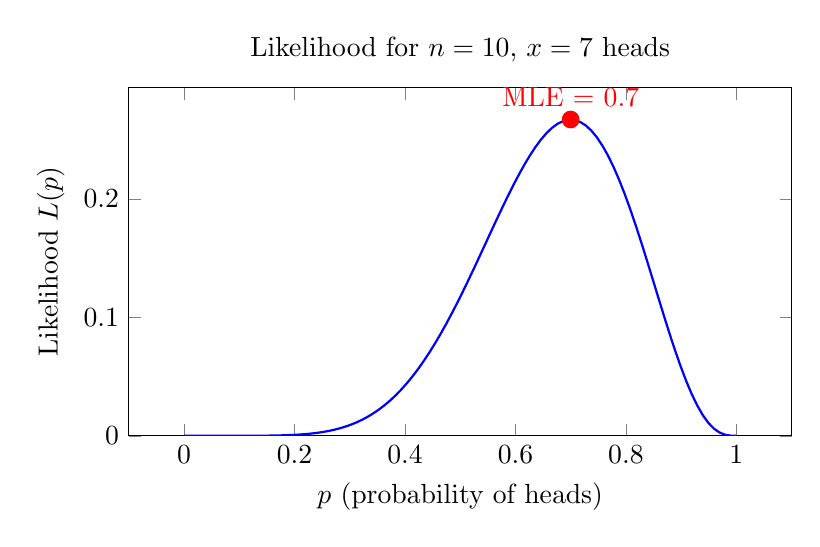
\begin{tikzpicture}
\begin{axis}[
    width=10cm,
    height=6cm,
    xlabel={$p$ (probability of heads)},
    ylabel={Likelihood $L(p)$},
    domain=0:1,
    samples=100,
    ymin=0,
    title={Likelihood for $n=10$, $x=7$ heads}
]
% Binomial likelihood: C(10,7) * p^7 * (1-p)^3
\addplot[thick, blue] {120 * x^7 * (1-x)^3};
\addplot[only marks, mark=*, mark size=3pt, red] coordinates {(0.7, 0.267)};
\node[above, red] at (axis cs:0.7,0.27) {MLE = 0.7};
\end{axis}
\end{tikzpicture}
\end{center}

\textbf{Observations:}
\begin{itemize}
\item Peak at $p = 7/10 = 0.7$ (intuitive!)
\item Fairly flat → lots of values plausible
\item Uncertainty due to small sample size
\end{itemize}
\end{frame}

% Maximum Likelihood Estimate
\begin{frame}{Maximum Likelihood Estimate (MLE)}

\begin{block}{Definition}
The \textbf{Maximum Likelihood Estimate (MLE)} is the parameter value that maximizes the likelihood function:
$$\hat{\theta}_{\text{MLE}} = \arg\max_{\theta} L(\theta \mid \text{data})$$
\end{block}

\vspace{0.3cm}

\textbf{For binomial:}
$$\hat{p} = \frac{x}{n}$$

(Can be shown by calculus: $\frac{dL}{dp} = 0$)

\vspace{0.3cm}

\textbf{Properties of MLE:}
\begin{itemize}
\item Intuitively sensible
\item Consistent: $\hat{\theta} \to \theta$ as $n \to \infty$
\item Asymptotically normal: $\hat{\theta} \sim N(\theta, \text{SE}^2)$ for large $n$
\item Basis for many statistical tests
\end{itemize}
\end{frame}

% Effect of Sample Size
\begin{frame}{Effect of Sample Size on Likelihood}

\textbf{Same proportion (70\% heads), different sample sizes:}

\vspace{0.3cm}

\begin{center}
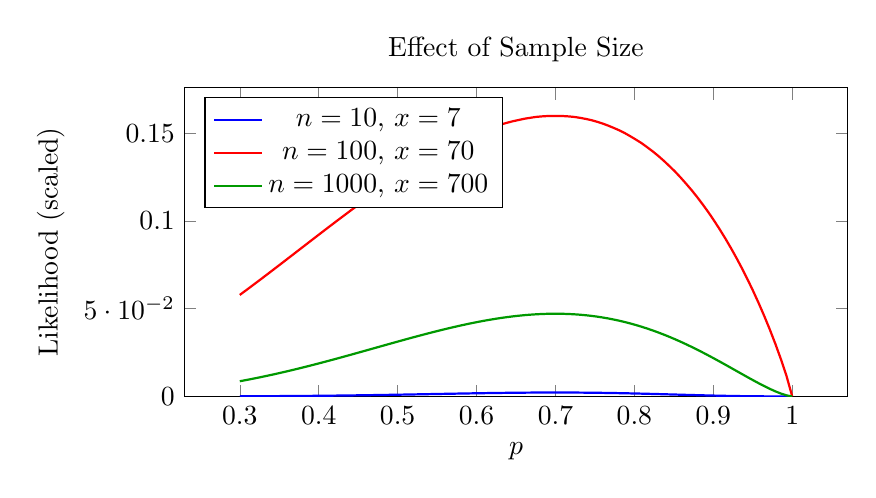
\begin{tikzpicture}
\begin{axis}[
    width=10cm,
    height=5.5cm,
    xlabel={$p$},
    ylabel={Likelihood (scaled)},
    domain=0.3:1,
    samples=100,
    legend pos=north west,
    ymin=0,
    title={Effect of Sample Size}
]
% n=10, x=7
\addplot[thick, blue] {x^7 * (1-x)^3};
\addlegendentry{$n=10$, $x=7$}

% n=100, x=70 (scaled to be visible)
\addplot[thick, red] {(x^70 * (1-x)^30)^0.03};
\addlegendentry{$n=100$, $x=70$}

% n=1000, x=700 (scaled to be visible)
\addplot[thick, green!60!black] {(x^700 * (1-x)^300)^0.005};
\addlegendentry{$n=1000$, $x=700$}
\end{axis}
\end{tikzpicture}
\end{center}

\textbf{Key observation:} Larger $n$ → sharper peak → more precision
\end{frame}

% Log-Likelihood
\begin{frame}{Log-Likelihood}

\textbf{Why use logarithms?}

\vspace{0.3cm}

\begin{block}{Definition}
$$\ell(\theta) = \log L(\theta)$$
\end{block}

\textbf{Advantages:}
\begin{enumerate}
\item Converts products to sums: $\log(ab) = \log a + \log b$
\item Easier to differentiate
\item Avoids numerical underflow (very small probabilities)
\item Same MLE: $\arg\max L = \arg\max \log L$
\end{enumerate}

\vspace{0.3cm}

\begin{exampleblock}{Binomial Log-Likelihood}
$$\ell(p) = \log\binom{n}{x} + x\log p + (n-x)\log(1-p)$$

Maximizing: $\frac{d\ell}{dp} = \frac{x}{p} - \frac{n-x}{1-p} = 0$ \\
Solving: $\hat{p} = \frac{x}{n}$
\end{exampleblock}
\end{frame}

% Biology Applications
\begin{frame}{Likelihood in Biology Research}

\textbf{Widespread applications:}

\vspace{0.3cm}

\begin{enumerate}
\item \textbf{Population genetics:} Estimate allele frequencies from genotype data

\vspace{0.2cm}
\item \textbf{Phylogenetics:} Find most likely evolutionary tree given DNA sequences

\vspace{0.2cm}
\item \textbf{Mark-recapture:} Estimate population size from capture data

\vspace{0.2cm}
\item \textbf{GLMs:} Generalized linear models (Poisson regression, logistic regression)

\vspace{0.2cm}
\item \textbf{Mixed models:} Estimate variance components in nested/hierarchical data

\vspace{0.2cm}
\item \textbf{Survival analysis:} Estimate hazard rates from time-to-event data
\end{enumerate}

\vspace{0.3cm}

\begin{alertblock}{}
\centering
MLE is the foundation of modern statistical inference!
\end{alertblock}
\end{frame}

% ============================================================================
% PART II: CONFIDENCE INTERVALS
% ============================================================================

\begin{frame}
\begin{center}
\Huge \textbf{Part II} \\
\vspace{0.5cm}
\LARGE Confidence Intervals
\vspace{0.5cm}

\large \textit{Quantifying uncertainty in our estimates}
\end{center}
\end{frame}

% The Logic
\begin{frame}{The Logic of Confidence Intervals}

\textbf{Recall from Day 2 (CLT):}
\begin{itemize}
\item Sample mean $\bar{x}$ varies across samples
\item Sampling distribution: $\bar{X} \sim N(\mu, \sigma^2/n)$
\item Standard Error: $SE = \sigma/\sqrt{n}$
\item 95\% of sample means fall within $\mu \pm 1.96 \times SE$
\end{itemize}

\vspace{0.3cm}

\begin{alertblock}{The Flip}
\textbf{Yesterday:} Given $\mu$, where is $\bar{x}$?

\textbf{Today:} Given $\bar{x}$, where is $\mu$?
\end{alertblock}

\vspace{0.3cm}

\textbf{Confidence Interval:}
$$\bar{x} \pm 1.96 \times SE$$

This interval will contain $\mu$ for 95\% of samples
\end{frame}

% Construction
\begin{frame}{Constructing a 95\% Confidence Interval}

\textbf{Case 1: Known $\sigma$ (rare in practice)}

$$\text{CI} = \bar{x} \pm 1.96 \times \frac{\sigma}{\sqrt{n}}$$

\vspace{0.3cm}

\textbf{Case 2: Unknown $\sigma$ (usual case)}

Use sample SD $s$ and $t$-distribution:
$$\text{CI} = \bar{x} \pm t_{\alpha/2, n-1} \times \frac{s}{\sqrt{n}}$$

where $t_{\alpha/2, n-1}$ is the critical value from $t$-distribution with $n-1$ degrees of freedom

\vspace{0.3cm}

\begin{exampleblock}{Example: Blood Pressure}
$n=25$, $\bar{x}=122$ mmHg, $s=15$ mmHg

\vspace{0.2cm}
$SE = 15/\sqrt{25} = 3$ mmHg \\
$t_{0.025, 24} = 2.064$ \\
$\text{CI} = 122 \pm 2.064 \times 3 = 122 \pm 6.2 = [115.8, 128.2]$
\end{exampleblock}
\end{frame}

% Interpretation
\begin{frame}{Interpreting Confidence Intervals}

\begin{block}{CORRECT Interpretation}
``We are 95\% confident that the interval $[115.8, 128.2]$ contains the true population mean $\mu$.''

\vspace{0.2cm}
Or: ``If we repeated this procedure many times, 95\% of the intervals would contain $\mu$.''
\end{block}

\vspace{0.3cm}

\begin{alertblock}{INCORRECT Interpretations}
\begin{itemize}
\item ✗ ``There's a 95\% probability that $\mu$ is in this interval'' \\
\small (Frequentist: $\mu$ is fixed, not random)

\item ✗ ``95\% of the data falls in this interval'' \\
\small (No! CI is about the parameter, not individual observations)

\item ✗ ``This specific interval has 95\% chance of containing $\mu$'' \\
\small (Once computed, either it does or doesn't—probability is about the procedure)
\end{itemize}
\end{alertblock}
\end{frame}

% Visualization
\begin{frame}{Visualizing Confidence Intervals}

\textbf{Simulation: 20 different samples, each gets a CI}

\vspace{0.2cm}

\begin{center}
\begin{tikzpicture}[scale=0.8]
\draw[thick, dashed, red] (5, 0) -- (5, 11) node[above] {True $\mu$};

\foreach \y/\color in {1/blue, 2/blue, 3/blue, 4/blue, 5/blue, 6/blue, 7/blue, 8/blue, 9/blue, 10/blue, 11/blue, 12/blue, 13/blue, 14/blue, 15/red, 16/blue, 17/blue, 18/blue, 19/blue, 20/blue} {
  \pgfmathsetmacro{\xmean}{5 + 0.6*rand}
  \pgfmathsetmacro{\xlower}{\xmean - 1}
  \pgfmathsetmacro{\xupper}{\xmean + 1}
  
  \draw[\color, thick] (\xlower, \y*0.5) -- (\xupper, \y*0.5);
  \fill[\color] (\xmean, \y*0.5) circle (2pt);
}

\draw[<->] (2, -0.5) -- (8, -0.5);
\node at (5, -1) {Parameter value};
\node[left] at (0, 5.5) {Different samples};
\end{tikzpicture}
\end{center}

\small \textcolor{blue}{19 intervals (95\%) contain $\mu$} \\
\textcolor{red}{1 interval (5\%) misses $\mu$}
\end{frame}

% Factors Affecting Width
\begin{frame}{Factors Affecting CI Width}

$$\text{Width} = 2 \times t_{\alpha/2} \times \frac{s}{\sqrt{n}}$$

\vspace{0.3cm}

\textbf{Narrower intervals (more precision) when:}

\begin{enumerate}
\item \textbf{Larger sample size ($n$):} Width $\propto 1/\sqrt{n}$
\begin{itemize}
\item Double the sample → width decreases by $\sqrt{2}$
\item To halve width, need 4× the data!
\end{itemize}

\vspace{0.2cm}
\item \textbf{Smaller variability ($s$):} More consistent measurements

\vspace{0.2cm}
\item \textbf{Lower confidence level:} 90\% CI narrower than 95\% CI
\begin{itemize}
\item But: trade-off between precision and confidence
\end{itemize}
\end{enumerate}

\vspace{0.3cm}

\begin{alertblock}{}
\centering
Can't have high precision and high confidence with small samples!
\end{alertblock}
\end{frame}

% Likelihood-based CI
\begin{frame}{Likelihood-Based Confidence Intervals}

\textbf{Alternative approach using likelihood:}

\vspace{0.3cm}

\begin{block}{Profile Likelihood CI}
Include all parameter values $\theta$ where:
$$-2[\ell(\theta) - \ell(\hat{\theta})] < \chi^2_{\alpha, 1}$$

For 95\% CI: $\chi^2_{0.05, 1} = 3.84$

\vspace{0.2cm}
Or approximately: $\ell(\theta) > \ell(\hat{\theta}) - 1.92$
\end{block}

\vspace{0.3cm}

\textbf{Advantages:}
\begin{itemize}
\item More accurate for small samples or non-normal distributions
\item Automatically respects parameter bounds (e.g., $p \in [0,1]$)
\item Basis for likelihood ratio tests
\end{itemize}

\vspace{0.2cm}

\textbf{In practice:} For large $n$, Wald and profile CIs are similar
\end{frame}

% ============================================================================
% PART III: HYPOTHESIS TESTING
% ============================================================================

\begin{frame}
\begin{center}
\Huge \textbf{Part III} \\
\vspace{0.5cm}
\LARGE Hypothesis Testing
\vspace{0.5cm}

\large \textit{Is the effect real, or just chance?}
\end{center}
\end{frame}

% The Logic
\begin{frame}{The Logic of Hypothesis Testing}

\textbf{Scientific question:} Does drug reduce blood pressure?

\vspace{0.3cm}

\textbf{Statistical approach:} Proof by contradiction

\begin{enumerate}
\item \textbf{Assume} drug has no effect (null hypothesis $H_0$)
\item Calculate: How likely is our observed data under $H_0$?
\item If very unlikely, reject $H_0$ (evidence for effect)
\item If not unlikely, fail to reject $H_0$ (insufficient evidence)
\end{enumerate}

\vspace{0.3cm}

\begin{alertblock}{Key Insight}
We \alert{never prove $H_0$ is true}—we only assess if data are \alert{incompatible} with $H_0$
\end{alertblock}

\vspace{0.2cm}

\textit{``Absence of evidence is not evidence of absence''}
\end{frame}

% Hypotheses
\begin{frame}{Null and Alternative Hypotheses}

\begin{block}{Null Hypothesis ($H_0$)}
Statement of \textbf{no effect} or \textbf{no difference}
\begin{itemize}
\item $H_0: \mu = \mu_0$ (mean equals specific value)
\item $H_0: \mu_1 = \mu_2$ (two groups have same mean)
\item $H_0: p = 0.5$ (proportion equals 0.5)
\end{itemize}
\end{block}

\begin{block}{Alternative Hypothesis ($H_A$ or $H_1$)}
What we suspect is true; contradicts $H_0$
\begin{itemize}
\item $H_A: \mu \neq \mu_0$ (two-sided: different in either direction)
\item $H_A: \mu > \mu_0$ (one-sided: specifically greater)
\item $H_A: \mu < \mu_0$ (one-sided: specifically less)
\end{itemize}
\end{block}

\vspace{0.2cm}

\begin{exampleblock}{Biology Example}
Test if knockout mice weigh less than wild-type: \\
$H_0: \mu_{\text{knockout}} = \mu_{\text{WT}}$ \quad vs. \quad $H_A: \mu_{\text{knockout}} < \mu_{\text{WT}}$
\end{exampleblock}
\end{frame}

% Test Statistic
\begin{frame}{Test Statistics}

\textbf{Need a number that measures deviation from $H_0$}

\vspace{0.3cm}

\begin{block}{General Form}
$$\text{Test Statistic} = \frac{\text{Estimate} - \text{Hypothesized value}}{\text{Standard Error}}$$
\end{block}

\vspace{0.3cm}

\textbf{Common test statistics:}

\begin{itemize}
\item \textbf{Z-statistic:} $Z = \frac{\bar{x} - \mu_0}{\sigma/\sqrt{n}}$ \quad (known $\sigma$)

\vspace{0.2cm}
\item \textbf{t-statistic:} $t = \frac{\bar{x} - \mu_0}{s/\sqrt{n}}$ \quad (unknown $\sigma$, use $s$)

\vspace{0.2cm}
\item \textbf{Two-sample t:} $t = \frac{\bar{x}_1 - \bar{x}_2}{\text{SE}_{\text{diff}}}$
\end{itemize}

\vspace{0.3cm}

\textbf{Under $H_0$:} Test statistic follows known distribution \\
\small (Z-distribution, t-distribution, etc.)
\end{frame}

% P-values
\begin{frame}{P-values}

\begin{block}{Definition}
\textbf{P-value} = Probability of observing data as extreme as (or more extreme than) what we actually observed, \alert{if $H_0$ were true}
$$p\text{-value} = P(\text{data as extreme} \mid H_0 \text{ true})$$
\end{block}

\vspace{0.3cm}

\textbf{Interpretation:}
\begin{itemize}
\item \textbf{Small p-value} (e.g., $p < 0.05$): Data are \alert{incompatible} with $H_0$ → reject $H_0$
\item \textbf{Large p-value} (e.g., $p > 0.05$): Data are \alert{consistent} with $H_0$ → fail to reject $H_0$
\end{itemize}

\vspace{0.3cm}

\begin{exampleblock}{Example}
$t = 2.5$, $p = 0.02$

\vspace{0.2cm}
\textit{``If there were truly no effect, we'd see a test statistic this large (or larger) only 2\% of the time. Since this is unlikely, we reject $H_0$."}
\end{exampleblock}
\end{frame}

% P-value Visualization
\begin{frame}{Visualizing P-values}

\textbf{Two-sided test:} $H_0: \mu = 0$, observed $t = 2.5$

\vspace{0.2cm}

\begin{center}
\begin{tikzpicture}[scale=0.9]
\begin{axis}[
    width=10cm,
    height=5.5cm,
    domain=-4:4,
    samples=100,
    xlabel={Test statistic},
    ylabel={Density},
    axis lines=center,
    ymin=0, ymax=0.45,
    xtick={-2.5, 0, 2.5},
    xticklabels={$-2.5$, $0$, $2.5$},
    title={Null distribution (t-distribution)}
]
% t-distribution with df=20
\addplot[thick, blue, domain=-4:4] {gamma(10.5)/(sqrt(20*pi)*gamma(10)) * (1 + x^2/20)^(-10.5)};

% Shade tails
\addplot[fill=red, opacity=0.3, domain=2.5:4] {gamma(10.5)/(sqrt(20*pi)*gamma(10)) * (1 + x^2/20)^(-10.5)} \closedcycle;
\addplot[fill=red, opacity=0.3, domain=-4:-2.5] {gamma(10.5)/(sqrt(20*pi)*gamma(10)) * (1 + x^2/20)^(-10.5)} \closedcycle;

% Mark observed value
\draw[thick, red, dashed] (axis cs:2.5,0) -- (axis cs:2.5,0.35);
\node[above, red] at (axis cs:2.5,0.35) {Observed};
\end{axis}
\end{tikzpicture}
\end{center}

\small \textcolor{red}{Shaded area = p-value} (probability in both tails)
\end{frame}

% What P-values Are NOT
\begin{frame}{What P-values Are NOT}

\begin{alertblock}{Common Misconceptions}

\textbf{P-value is NOT:}

\begin{itemize}
\item ✗ Probability that $H_0$ is true \\
\small (We condition on $H_0$ being true to calculate p!)

\vspace{0.2cm}
\item ✗ Probability that results are due to chance \\
\small (Everything has chance involved; p quantifies compatibility with $H_0$)

\vspace{0.2cm}
\item ✗ Probability of making a mistake \\
\small (That's $\alpha$, not p)

\vspace{0.2cm}
\item ✗ Size of the effect \\
\small (Large effect with large n → small p; small effect with huge n → small p)

\vspace{0.2cm}
\item ✗ Importance of the finding \\
\small (Statistical significance $\neq$ practical significance)
\end{itemize}
\end{alertblock}

\vspace{0.2cm}

\textbf{P-value IS:} Measure of compatibility between data and $H_0$
\end{frame}

% Decision Rule
\begin{frame}{Decision Rules and Significance Level}

\begin{block}{Significance Level ($\alpha$)}
Threshold for rejecting $H_0$ (conventionally 0.05)

\vspace{0.2cm}
\textbf{Decision rule:}
\begin{itemize}
\item If $p < \alpha$: Reject $H_0$ (result is ``statistically significant'')
\item If $p \geq \alpha$: Fail to reject $H_0$ (result is ``not significant'')
\end{itemize}
\end{block}

\vspace{0.3cm}

\begin{alertblock}{Important Notes}
\begin{itemize}
\item $\alpha = 0.05$ is arbitrary! (R.A. Fisher's convention)
\item Don't treat $p = 0.049$ differently from $p = 0.051$
\item Better: Report exact p-value, let readers judge
\item Even better: Report effect sizes with CIs!
\end{itemize}
\end{alertblock}

\vspace{0.2cm}

\textbf{Modern practice:} De-emphasize ``significant'' / ``not significant'' binary
\end{frame}

% One-sided vs Two-sided
\begin{frame}{One-Sided vs. Two-Sided Tests}

\begin{columns}[T]
\begin{column}{0.48\textwidth}
\begin{block}{Two-Sided}
$H_0: \mu = \mu_0$ \\
$H_A: \mu \neq \mu_0$

\vspace{0.2cm}
Detect difference in \textbf{either direction}

\vspace{0.2cm}
P-value: sum of both tails

\vspace{0.2cm}
\end{block}
\end{column}
\end{columns}
\end{frame}
\end{document}
